
\subsection{Data Link}
  \begin{frame}
    \frametitle{Aims}
      \begin{itemize}
        \item Interface network layer,\pause
        \item Delivery to unique(?) hardware addresses,\pause
        \item Framing,\pause
        \item Data transfer
      \end{itemize}
  \end{frame}
  \begin{frame}
    \frametitle{Layer composition (of its two sublayers)}
      \begin{enumerate}
        \item Logical Link Control (LLC):
          \begin{itemize}
            \item end to end flow control
            \item end to end error control
            \item (transmitting/receiving) protocols, over MAC sublayer, multiplexing
          \end{itemize}\pause
        \item Media Access Control (MAC):
          \begin{itemize}
            \item physical (hardware) addressing
            \item collision detection and retransmission
            \item data packet scheduling (and queuing)
            \item QoS
            \item VLAN
          \end{itemize}
      \end{enumerate}
  \end{frame}
  \begin{frame}
    \frametitle{Carrier Sense Multiple Access with Collision Avoidance}
    \begin{figure}[t]
      \centering
      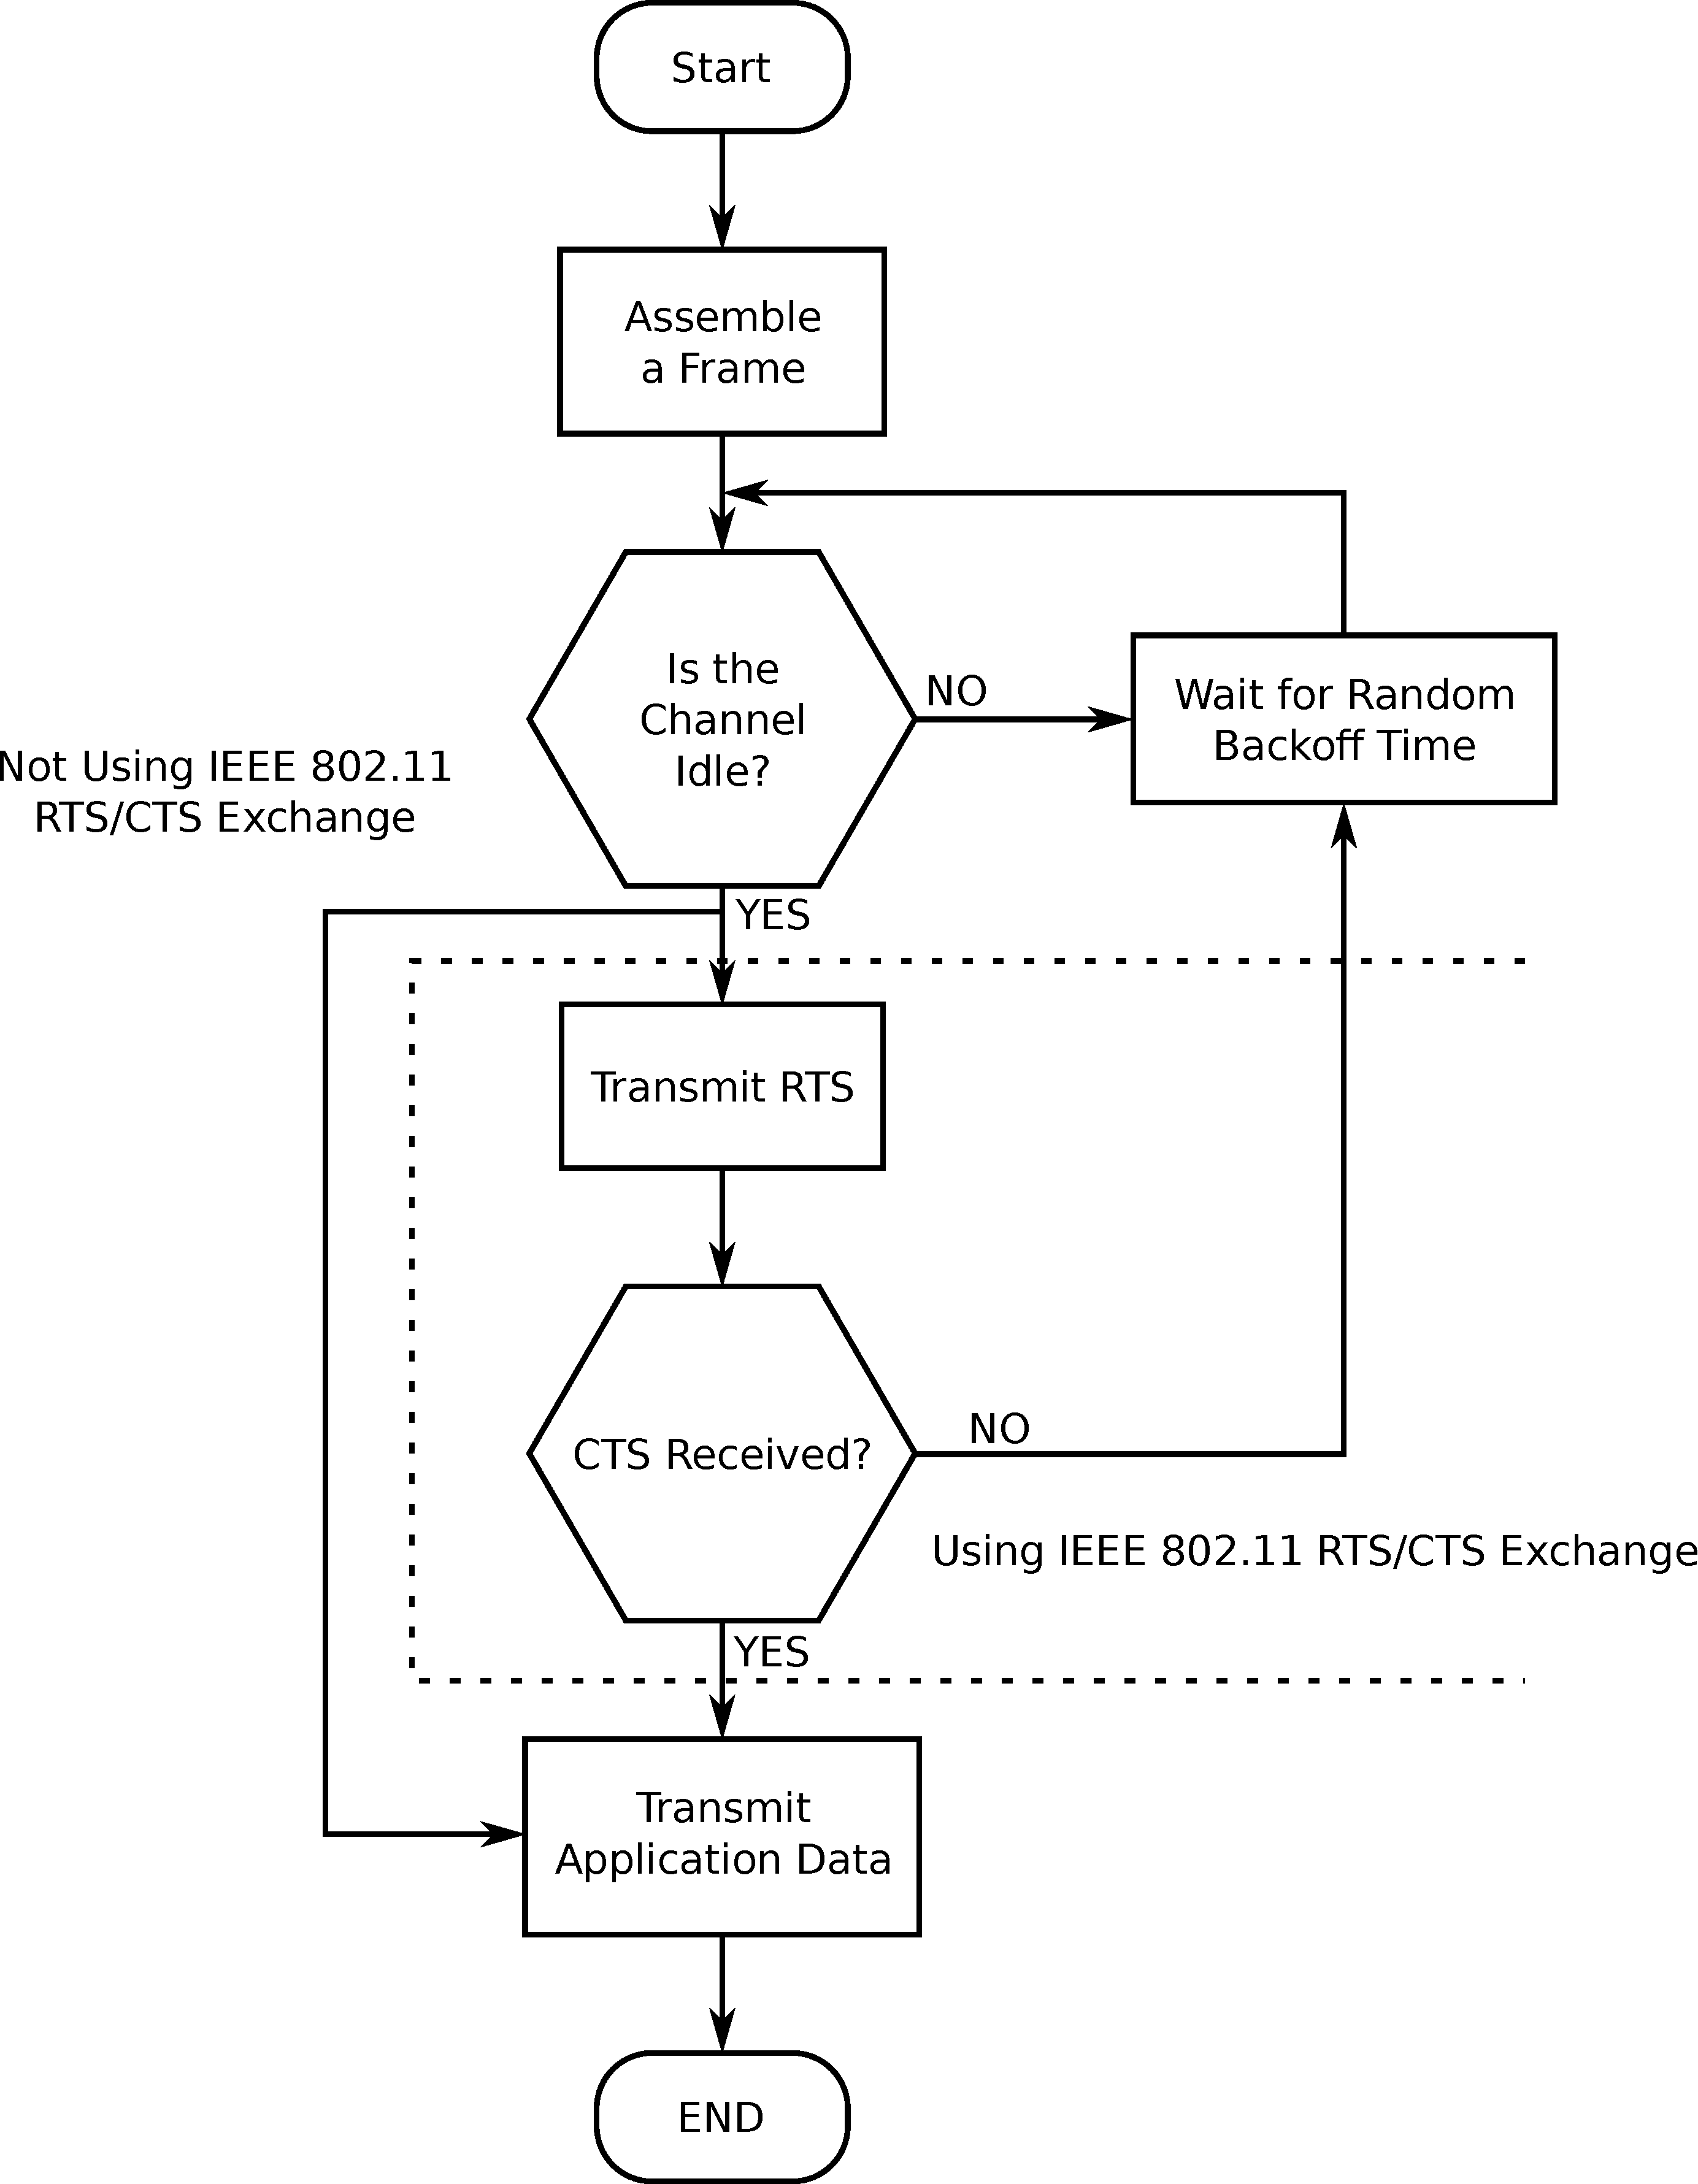
\includegraphics[height=6cm]{./imgs/csma_ca.pdf}
      \caption{\color{blue}\href{https://en.wikipedia.org/wiki/File:Csma_ca.svg}{CSMA CA}}
      \label{fig:csma_ca}
    \end{figure}
    \end{frame}
  \begin{frame}
    \frametitle{Layer 2 Ethernet packet}
      \begin{figure}[h]
      \centering
      \begin{tabular}{|c|c|c|c|c|c|c|c|c|}
        \hline
        \multicolumn{3}{|c|}{MAC dest. (\color{blue}6\color{black})} & \multicolumn{3}{|c|}{MAC src. (\color{blue}6\color{black})} & \multicolumn{2}{|c|}{\color{brown}VLAN tag* (\color{blue}4\color{brown})\color{black}} & Ethertype (\color{blue}2\color{black}) \\ \hline
        \multicolumn{6}{|c|}{Payload (\color{blue}42-1500\color{black})} & \multicolumn{3}{|c|}{Frame check sequence (\color{blue}4\color{black})}\\ \hline
      \end{tabular}
      \caption{Layer 2 Ethernet packet}
      \label{fig:eth_packet}
    \end{figure}
    \hfill \color{brown}optional\color{black}, Content (\color{blue}size in bytes\color{black})
    \begin{figure}[h]
      \centering
      \begin{tabular}{|c|c|}
        \hline
        \textbf{Ethertype 0x} & \textbf{Protocol} \\ \hline
        0800 & IPv4 \\ \hline
        0806 & ARP \\ \hline
        0842 & Wake-on-LAN \\ \hline
        86dd & IPv6 \\ \hline
      \end{tabular}
      \caption{Data received with MDPC}
      \label{fig:eth_type}
    \end{figure}
  \end{frame}


  \begin{frame}
    \frametitle{ARP example}
      \begin{figure}
      \centering
      \resizebox{11.5cm}{!} {
        \begin{tabular}{lcccccccccccccccc}
          \textbf{0000} & ff & ff & ff & ff & ff & ff & fa & ba & 00 & ab & ab & af & 08 & 06 & 00 & 01 \\
          \textbf{0010} & 08 & 00 & 06 & 04 & 00 & 01 & fa & ba & 00 & ab & ab & af & ac & 11 & 22 & 37 \\
          \textbf{0020} & 00 & 00 & 00 & 00 & 00 & 00 & ac & 11 & 00 & f9 & 00 & 00 & 00 & 00 & 00 & 00 \\
          \textbf{0030} & 00 & 00 & 00 & 00 & 00 & 00 & 00 & 00 & 00 & 00 & 00 & 00 \\
        \end{tabular}
      }
      \caption{ARP request}
      \label{fig:arp_packet_ex}
    \end{figure}
        MAC address destination MAC address source Ethertype Hardware type Protocol type OpCode (1 request, 2 reply) IP address source IP address destination
  \end{frame}

  \begin{frame}
    \frametitle{ARP example}
      \begin{figure}
      \centering
      \resizebox{11.5cm}{!} {
        \begin{tabular}{lcccccccccccccccc}
          \textbf{0000} & \color{red}ff & \color{red}ff & \color{red}ff & \color{red}ff & \color{red}ff & \color{red}ff & \color{Marroon}fa & \color{Marroon}ba & \color{Marroon}00 & \color{Marroon}ab & \color{Marroon}ab & \color{Marroon}af & \color{blue}08 & \color{blue}06 & \color{magenta}00 & \color{magenta}01 \\
          \textbf{0010} & \color{OliveGreen}08 & \color{OliveGreen}00 & \color{gray}06 & \color{gray}04 & \color{fuchsia}00 & \color{fuchsia}01 & \color{Marroon}fa & \color{Marroon}ba & \color{Marroon}00 & \color{Marroon}ab & \color{Marroon}ab & \color{Marroon}af & \color{brown}ac & \color{brown}11 & \color{brown}22 & \color{brown}37 \\
          \textbf{0020} & \color{red}00 & \color{red}00 & \color{red}00 & \color{red}00 & \color{red}00 & \color{red}00 & \color{orange}ac & \color{orange}11 & \color{orange}00 & \color{orange}f9 & 00 & 00 & 00 & 00 & 00 & 00 \\
          \textbf{0030} & 00 & 00 & 00 & 00 & 00 & 00 & 00 & 00 & 00 & 00 & 00 & 00 \\
        \end{tabular}
      }
      \caption{ARP request}
      \label{fig:arp_req_ex-colored}
    \end{figure}
    \color{red}MAC address destination \color{Marroon}MAC address source \color{blue}Ethertype \color{magenta}Hardware type \color{OliveGreen}Protocol type \color{fuchsia}OpCode (1 request, 2 reply) \color{brown} IP address source \color{orange} IP address destination
  \end{frame}
  \begin{frame}
    \frametitle{ARP example}
      \begin{figure}
      \centering
      \resizebox{11.5cm}{!} {
        \begin{tabular}{lcccccccccccccccc}
          \textbf{0000} & fa & ba & 00 & ab & ab & af & be & be & 00 & 00 & eb & eb & 08 & 06 & 00 & 01 \\
          \textbf{0010} & 08 & 00 & 06 & 04 & 00 & 01 & be & be & 00 & 00 & eb & eb & ac & 11 & 00 & f9 \\
          \textbf{0020} & fa & ba & 00 & ab & ab & af & ac & 11 & 22 & 37 & 00 & 00 & 00 & 00 & 00 & 00 \\
          \textbf{0030} & 00 & 00 & 00 & 00 & 00 & 00 & 00 & 00 & 00 & 00 & 00 & 00 \\
        \end{tabular}
      }
      \caption{ARP reply}
      \label{fig:arp_rep_ex}
    \end{figure}
        MAC address destination MAC address source Ethertype Hardware type Protocol type OpCode (1 request, 2 reply) IP address source IP address destination
  \end{frame}
  \begin{frame}
    \frametitle{ARP example}
      \begin{figure}
      \centering
      \resizebox{11.5cm}{!} {
        \begin{tabular}{lcccccccccccccccc}
          \textbf{0000} & \color{red}fa & \color{red}ba & \color{red}00 & \color{red}ab & \color{red}ab & \color{red}af & \color{Marroon}be & \color{Marroon}be & \color{Marroon}00 & \color{Marroon}00 & \color{Marroon}eb & \color{Marroon}eb & \color{blue}08 & \color{blue}06 & \color{magenta}00 & \color{magenta}01 \\
          \textbf{0010} & \color{OliveGreen}08 & \color{OliveGreen}00 & \color{gray}06 & \color{gray}04 & \color{fuchsia}00 & \color{fuchsia}01 & \color{Marroon}be & \color{Marroon}be & \color{Marroon}00 & \color{Marroon}00 & \color{Marroon}eb & \color{Marroon}eb & \color{brown}ac & \color{brown}11 & \color{brown}00 & \color{brown}f9 \\
          \textbf{0020} & \color{red}fa & \color{red}ba & \color{red}00 & \color{red}ab & \color{red}ab & \color{red}af & \color{orange}ac & \color{orange}11 & \color{orange}22 & \color{orange}37 & 00 & 00 & 00 & 00 & 00 & 00 \\
          \textbf{0030} & 00 & 00 & 00 & 00 & 00 & 00 & 00 & 00 & 00 & 00 & 00 & 00 \\
        \end{tabular}
      }
      \caption{ARP reply}
      \label{fig:arp_rep_ex-colored}
    \end{figure}
    \color{red}MAC address destination \color{Marroon}MAC address source \color{blue}Ethertype \color{magenta}Hardware type \color{OliveGreen}Protocol type \color{fuchsia}OpCode (1 request, 2 reply) \color{brown} IP address source \color{orange} IP address destination
  \end{frame}